\documentclass[../TDE8_filtrage.tex]{subfiles}%

\begin{document}
\section[s]"2"{Filtre de \textsc{Wien}}
\enonce{%
	\noindent
	\begin{minipage}[c]{.3\linewidth}
		On s'intéresse au filtre de \textsc{Wien}, représenté ci-contre.
	\end{minipage}
	\hfill
	\begin{minipage}[c]{.7\linewidth}
		~
		\begin{center}
			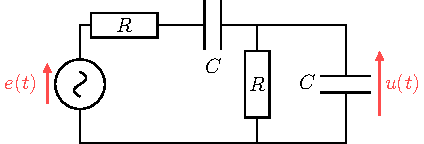
\includegraphics[width=.6\textwidth]{wien_plain}
		\end{center}
	\end{minipage}
}

\QR{%
	Par analyse des comportements asymptotiques, déterminer le type de filtre dont
	il s'agit.
}{%
	~
	\vspace{-15pt}
	\smallbreak
	\noindent
	\begin{isd}[sidebyside align=top]
		\tcbsubtitle{\fatbox{Basses fréquences}}
		\begin{center}
			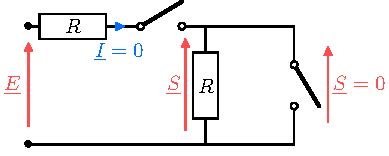
\includegraphics[width=\linewidth]{wien_bf}
		\end{center}
		Dans la limite très basses fréquences, les condensateurs sont cette fois
		équivalents à des interrupteurs ouverts. Aucun courant ne circule dans les
		résistances, et on a donc également $\Su = 0$.
		\tcblower
		\tcbsubtitle{\fatbox{Hautes fréquences}}
		\begin{center}
			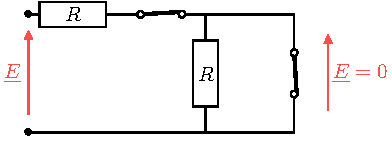
\includegraphics[width=\linewidth]{wien_hf}
		\end{center}
		\vspace{-15pt}
		Dans la limite très hautes fréquences, les condensateurs sont
		équivalents à des fils, donc $\Su = 0$.
	\end{isd}
	Selon toute vraisemblance, c'est donc un filtre \textbf{passe-bande}.
}

\QR{%
	Déterminer la fonction de transfert $\Hu$ du filtre.
}{%
	Notons $\Zu$ l'impédance et $\Yu$ l'admittance de l'association
	RC parallèle. En utilisant cette impédance, on reconnaît un pont
	diviseur de tension~:
	\begin{center}
		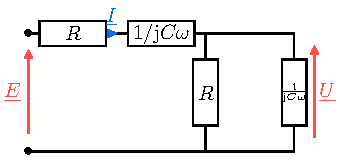
\includegraphics[scale=1]{wien_cplx}
	\end{center}
	\begin{gather*}
		\Hu = \frac{\Su}{\Eu} = \frac{\Zu}{R + \dfrac{1}{\jj
				C\w} + \Zu}
		\Lra
		\Hu
		= \frac{1}{1 + \left(R + \dfrac{1}{\jj C\w}\right)\Yu}
		= \frac{1}{1 + \left(R + \dfrac{1}{\jj C\w}\right)\left(
			\dfrac{1}{R} + \jj C\w\right)}\\
		\Lra
		\boxed{\Hu = \frac{1}{3+\jj\left(RC\w - \dfrac{1}{RC\w}\right)}}
	\end{gather*}
}

\QR{%
	On pose $\w_0 = 1/RC$ et $x=\w/\w_0$. Écrire la fonction de transfert
	sous la forme
	\[ \Hu = \frac{H_0}{1 + \jj Q \left( x - \dfrac{1}{x} \right)}\]
	en précisant les valeurs de $H_0$ et $Q$.
}{%
	En factorisant par 3 et en utilisant les notations introduites dans
	l'énoncé, on trouve
	\begin{gather*}
		\Hu
		= \frac{1/3}{1 + \dfrac{\jj}{3} \left( x - \dfrac{1}{x} \right)}
		\Lra
		\boxed{
			\Hu = \frac{H_0}{1 + \jj Q \left( x - \dfrac{1}{x} \right)}}
		\qavec
		\boxed{
			\left\{
			\begin{array}{rcl}
				H_0 & = & 1/3 \\
				Q   & = & 1/3
			\end{array}
			\right.
		}
	\end{gather*}
}

\QR{%
	Calculer simplement le gain maximal du filtre, puis le gain maximal en
	décibels, et le déphasage correspondant à ce maximum.
}{%
	Le gain en amplitude du filtre est défini par
	\[G = \abs{\Hu} = \frac{H_0}{\sqrt{1 + Q^2 \left( x - \dfrac{1}{x}
				\right)^2}}\]
	Il est maximal lorsque le dénominateur est minimal, c'est-à-dire lorsque
	le terme entre parenthèses s'annule. Cela correspond à $x=1$, d'où le
	gain maximal $\mathbf{G_{\max} = 1/3}$. \bigbreak
	Le gain \textbf{en décibels} du filtre est défini par
	\[G_{\rm dB} = 20\log(\abs{\Hu})\]
	et on trouve donc $\mathbf{G_{\rm dB, max} = 20\log(1/3) =
			\SI{-9.5}{dB}}$. De plus, en $x = 1$ la fonction de transfert est
	réelle, donc son argument est nul~: à la pulsation $\w_0$, la sortie et
	l'entrée ne sont donc pas déphasées.
}

\QR{%
	Représenter le diagramme de \textsc{Bode} asymptotique du filtre et en
	déduire qualitativement le tracé réel.
}{%
	Dans la limite très basses fréquences, la fonction de transfert est
	équivalente à
	\[\Hu
		\underset{x\ra0}{\sim} \frac{H_0}{-\jj Q/x}
		= \jj \frac{H_0}{Q} x
		\qdonc
		\left\{
		\begin{array}{rcl}
			G_{\dB} & = & 20\log\abs{\Hu}
			\underset{x\ra0}{\sim} 20 \log x       \\
			\f      & = & \arg \Hu = \frac{\pi}{2}
		\end{array}
		\right.
	\]
	De même, dans la limite très hautes fréquences, on a
	\[\Hu
		\underset{x\ra\infty}{\sim} \frac{H_0}{\jj Qx}
		= -\jj \frac{H_0}{Q} \frac{1}{x}
		\qdonc
		\left\{
		\begin{array}{rcl}
			G_{\dB} & = & 20\log\abs{\Hu}
			\underset{x\ra0}{\sim} -20 \log x       \\
			\f      & = & \arg \Hu = -\frac{\pi}{2}
		\end{array}
		\right.
	\]

	Ainsi, le diagramme de \textsc{Bode} asymptotique en gain compte
	\textbf{deux asymptotes de pentes $\mathbf{\pm}$ \SI{20}{dB/décade}
		passant par $\mathbf{G_{\dB} = 0}$ pour $\mathbf{x=1}$}, alors que le
	diagramme asymptotique en phase compte \textbf{deux asymptotes
		horizontales de hauteurs $\mathbf{\pm \pi/2}$}. \bigbreak
	Pour tracer l'allure du diagramme réel, on utilise en plus les résultats
	de la question précédente qui indique que la courbe réelle passe par
	$G_{\dB} = \SI{-9.5}{dB}$ en $x=1$, alors que la courbe de phase réelle
	passe par $0$ en $x=1$~; d'où les diagrammes ci-dessous.

	\begin{center}
		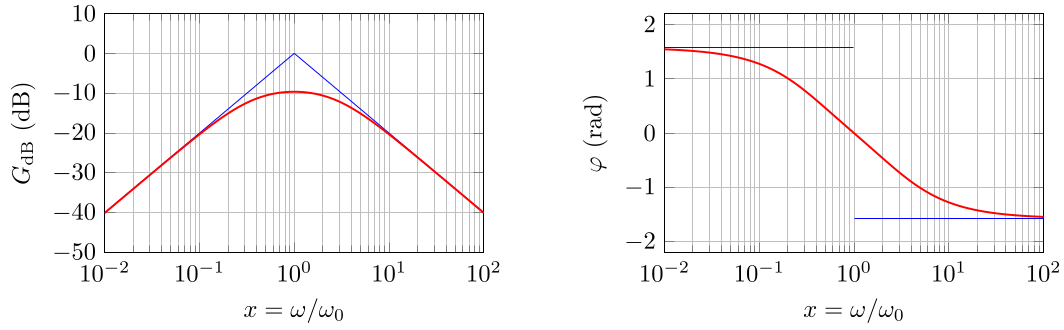
\includegraphics[width=\linewidth]{wien_bode}
	\end{center}
}

\QR{%
	Calculer la pulsation propre $\w_0$ pour $R = \SI{1.0}{k\Omega}$ et $C
		= \SI{500}{nF}$. Donner le signal de sortie du filtre si le signal
	d'entrée est
	\[e(t) = E_0 + E_0\cos(\wt) + E_0\cos(10\wt) + E_0\cos(100\wt)\]
	avec $E_0 = \SI{10}{V}$ et $\w = \SI{200}{rad.s^{-1}}$.
}{%
	Numériquement, on trouve $\w_0 = \SI{2.0e3}{rad.s^{-1}}$. Comme le
	diagramme de \textsc{Bode} réel n'est pas donné dans l'énoncé, on peut
	au choix utiliser la fonction de transfert ou raisonner sur le diagramme
	asymptotique. Étudions le signal de sortie du filtre associé à chaque
	composante du signal d'entrée~:
	\begin{itemize}
		\item Le terme continu est complètement coupé par le filtre~;
		\item Le terme de pulsation $\w = \w_0/10$ se trouve une décade
		      en-dessous de la pulsation propre~: avec le diagramme
		      asymptotique il est donc atténué de \SI{20}{dB}, ce qui
		      correspond à un facteur 10 en amplitude, et déphasé d'environ
		      \SI{1.2}{rad} si le diagramme réel tracé~;
		\item Le terme de pulsation $10\w = \w_0$ est à la pulsation propre
		      du filtre~: il n'est pas déphasé mais seulement atténué d'un
		      facteur 1/3 (gain maximal)~;
		\item Le terme à la pulsation $100\w = 10\w_0$ est une décade
		      au-dessus de la pulsation propre~: il est atténué comme le
		      premier terme d'un facteur 10 en amplitude, et déphasé d'environ
		      \SI{-1.2}{rad}. Ainsi,
	\end{itemize}
	\[\boxed{
			s(t) =
			\frac{E_0}{10}\cos (\wt - \num{1.2}) +
			\frac{E_0}{3}\cos(10\wt) +
			\frac{E_0}{10}\cos (100\wt + \num{1.2})
		}\]
}

\end{document}
